%
% This is a borrowed LaTeX template file for lecture notes for CS267,
% Applications of Parallel Computing, UCBerkeley EECS Department.
% Now being used for CMU's 10725 Fall 2012 Optimization course
% taught by Geoff Gordon and Ryan Tibshirani.  When preparing 
% LaTeX notes for this class, please use this template.
%
% To familiarize yourself with this template, the body contains
% some examples of its use.  Look them over.  Then you can
% run LaTeX on this file.  After you have LaTeXed this file then
% you can look over the result either by printing it out with
% dvips or using xdvi. "pdflatex template.tex" should also work.
%

\documentclass[twoside]{article}
\setlength{\oddsidemargin}{0.25 in}
\setlength{\evensidemargin}{-0.25 in}
\setlength{\topmargin}{-0.6 in}
\setlength{\textwidth}{6.5 in}
\setlength{\textheight}{8.5 in}
\setlength{\headsep}{0.75 in}
\setlength{\parindent}{0 in}
\setlength{\parskip}{0.1 in}

%
% ADD PACKAGES here:
%
\usepackage{float}
\usepackage{epstopdf} 
\usepackage{amsmath,amsfonts,graphicx}
\usepackage[utf8]{inputenc}

%
% The following commands set up the lecnum (lecture number)
% counter and make various numbering schemes work relative
% to the lecture number.
%
\newcounter{lecnum}
\renewcommand{\thepage}{\thelecnum-\arabic{page}}
\renewcommand{\thesection}{\thelecnum.\arabic{section}}
\renewcommand{\theequation}{\thelecnum.\arabic{equation}}
\renewcommand{\thefigure}{\thelecnum.\arabic{figure}}
\renewcommand{\thetable}{\thelecnum.\arabic{table}}

%
% The following macro is used to generate the header.
%
\newcommand{\lecture}[4]{
   \pagestyle{myheadings}
   \thispagestyle{plain}
   \newpage
   \setcounter{lecnum}{#1}
   \setcounter{page}{1}
   \noindent
   \begin{center}
   \framebox{
      \vbox{\vspace{2mm}
    \hbox to 6.28in { {\bf Web Information Retrieval
	\hfill Spring 2018} }
       \vspace{4mm}
       \hbox to 6.28in { {\Large \hfill #2  \hfill} }
       \vspace{2mm}
       \hbox to 6.28in { { \textbf{Members}: \textit{#3} \hfill  #4} }
      \vspace{2mm}}
   }
   \end{center}
   

   %{\bf Note}: {\it LaTeX template courtesy of UC Berkeley EECS dept.}

   \vspace*{4mm}
}
%
% Convention for citations is authors' initials followed by the year.
% For example, to cite a paper by Leighton and Maggs you would type
% \cite{LM89}, and to cite a paper by Strassen you would type \cite{S69}.
% (To avoid bibliography problems, for now we redefine the \cite command.)
% Also commands that create a suitable format for the reference list.
\renewcommand{\cite}[1]{[#1]}
\def\beginrefs{\begin{list}%
        {[\arabic{equation}]}{\usecounter{equation}
         \setlength{\leftmargin}{2.0truecm}\setlength{\labelsep}{0.4truecm}%
         \setlength{\labelwidth}{1.6truecm}}}
\def\endrefs{\end{list}}
\def\bibentry#1{\item[\hbox{[#1]}]}

%Use this command for a figure; it puts a figure in wherever you want it.
%usage: \fig{ NUMBER}{SPACE-IN-INCHES}{CAPTION}
\newcommand{\fig}[1]{
			\begin{center}
			#1
			\end{center}
	}
% Use these for theorems, lemmas, proofs, etc.
\newtheorem{theorem}{Theorem}[lecnum]
\newtheorem{lemma}[theorem]{Lemma}
\newtheorem{proposition}[theorem]{Proposition}
\newtheorem{claim}[theorem]{Claim}
\newtheorem{corollary}[theorem]{Corollary}
\newtheorem{definition}[theorem]{Definition}
\newenvironment{proof}{{\bf Proof:}}{\hfill\rule{2mm}{2mm}}

% **** IF YOU WANT TO DEFINE ADDITIONAL MACROS FOR YOURSELF, PUT THEM HERE:

\newcommand\E{\mathbb{E}}

\begin{document}
\lecture{1}{WIR Final Relation}{Angelo Catalani, Valerio Colitta, Alessandro Lo Presti}

\section{Introduction}
The vector space model is characterized by the representation of documents and queries as vectors and the cosine similarity to compute the similarity score between them.\\This means that if the distinct terms in a given collection are n, each document is a n-dimensional vector.\\The VSM assumes that for each term $t_i$ there exists a vector $\vec{t_i}$ in the vector space the represents it, and these vectors form the space basis.\\This leads to the fact, each document (or query) is a linear combination of the vectors $t_i$ : $d_k = \sum\limits_{i=1}^n w_i\vec{t_i}$ , where $w_i$ is the tf-idf score for the term $t_i$ in the document : $d_k$  .\\The underlying assumption is the pairwise orthogonality of terms vector that brings to the conclusion there can not be any semantic correlation between terms.\\The GVSM extends the VSM by non considering terms vectors orthogonal and computing the similarity score between terms according the following formula : $score(\vec{d},\vec{q}) = \frac{\mathop{\sum_{j=1}^{n'}\sum_{i=1}^{n'}}\vec{t_i}\cdot\vec{t_j}\cdot d[i]\cdot q[j] }{||\vec{d_k} ||\cdot||\vec{q} ||}$.\\It is interesting to note this formula reduces to the classical cosine similarity assuming pairwise orthogonality of the terms vectors because that product is always zero except when they are the same($i=j$).\\The dot product of the terms is their semantic correlation.

\section{Generalized Vector Space Model}
The paper\cite{LM89} taken into consideration, considered documents to be $n' = n\cdot(n-1)/2$ dimensional vectors where, each dimension stands for a distinct pair of terms and all the distinct terms are $n$.\\In particular for a given document $d_k$, the entry $d_k[i][j] = d_k(t_i,t_j) = (tf-idf(t_i,d_k)+tf-idf(t_j,d_k)) \cdot \vec{t_i}\cdot\vec{t_j}$.\\The dimension is not $n*n$ because it is assumed the similarity function between terms is symmetric, so that the entry  $d_k(t_i,t_j) = d_k(t_j,t_i)$.\\Finally, the score function has been defined as : $score(\vec{d},\vec{q}) = \frac{\mathop{\sum_{j=1}^{n'}\sum_{i=1}^{n'}}d_k[i][j]\cdot q[i][j] }{||\vec{d_k} ||\cdot||\vec{q} ||}$
\subsection{Implementation}
The first task has consisted of parsing the dataset and build a matrix of tf-idf scores where each row index is the documentID and each col is the termID.\\This function is not performance critical because our dataset is relatively small.\\The second task has been the implementation of the function, that takes as parameters 2 rows of that matrix and a term-to-term similarity function and computes the score function described above.\\The first problem was the fact that the original formulation consists of a nested loop iterating over all the possible terms couples with a complexity of $O(n^2)$ that executed over all the queries and documents, causes a serious performance penalty.\\To deal with this issue, an approximated function has been introduced that iterates only over the terms that appears in the document or in the query.\\This approximation results in raising the final score with respect to the original one, because: 
\begin{enumerate}
\item the numerator is the same since it is different from zero only when in the couple of terms considered, at least one belongs to the document and the other, but also the same, to the query.
\item the denominator however is different from zero even if one terms belongs to the document (or query), and the other does not.
\end{enumerate}
The approximated solution performed in less time with coherent results.\\However, the second bottle neck is the computation of the term-to-term similarity function, whose description is delayed to the next section.

\section{Similarity Function}
\section{Dataset and Result}
The first dataset is made of
\begin{enumerate}
\item Documents : $11429$
\item Queries : $90$
\item Distinct terms : $11945$
\end{enumerate}
This dataset has associated a ground truth file with the relevant documentIDs associated to each query.\\Since the computation of the score function is performance demanding the tests have been conducted after resizing the dataset.\\The precision-recall plot is calculated as an average of the precision for a given recall level for the number  query considered.\\In particular 10 recall levels have been considered : $ 0.1, 0.2, ... , 1.0 $.\\In addition to this, it has been executed a test also on the classical cosine similarity where it has been possible to consider the whole dataset since each computation has a linear complexity.
\begin{figure}[H]
\centering
        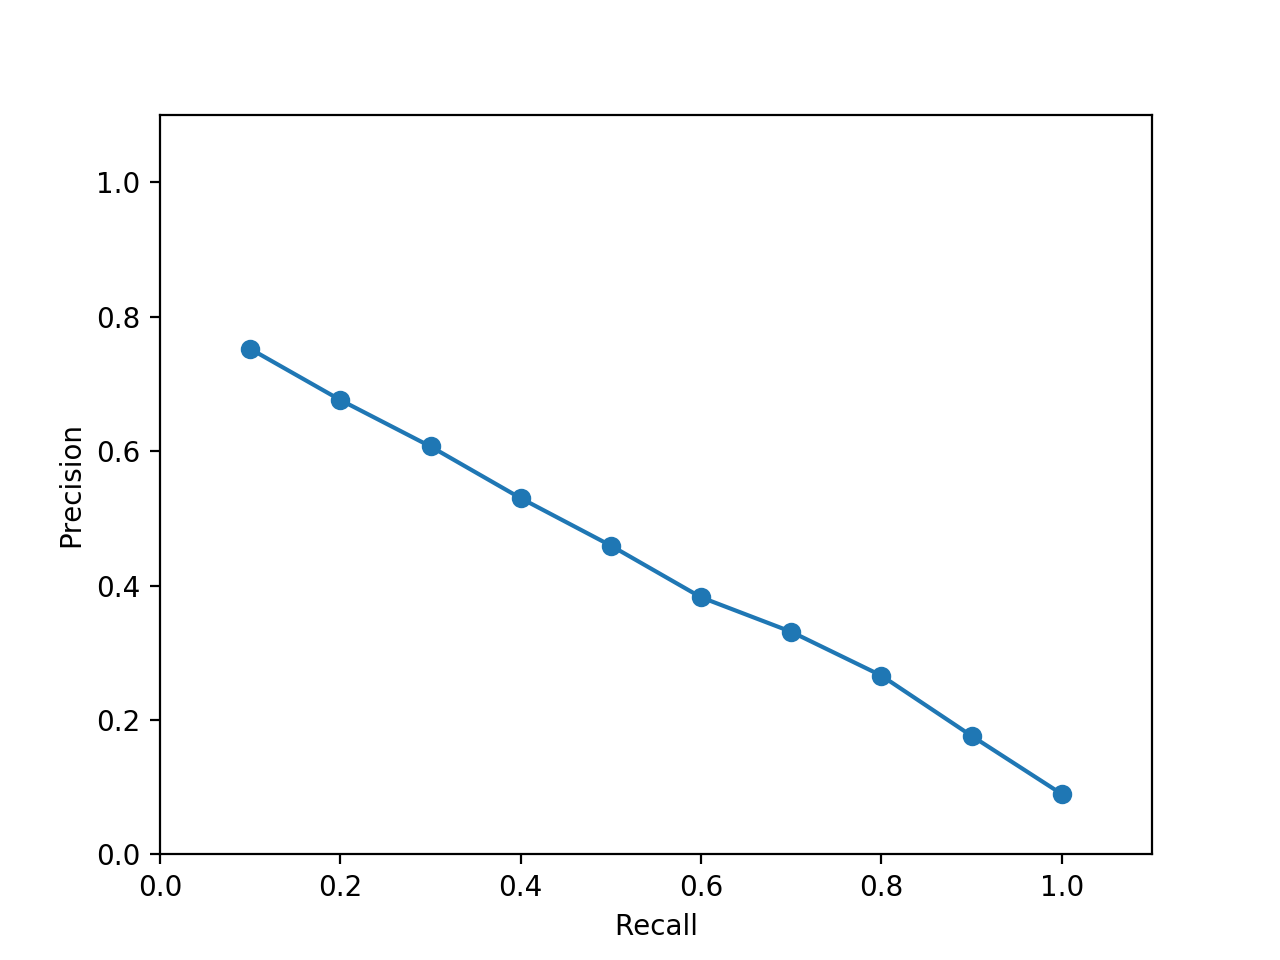
\includegraphics[totalheight=8cm]{cs.png}
    \caption{Precision-Recall Cosine-Similarity}
    \label{fig:plot1}
\end{figure}

%
%\begin{figure}[H]
%\centering
%        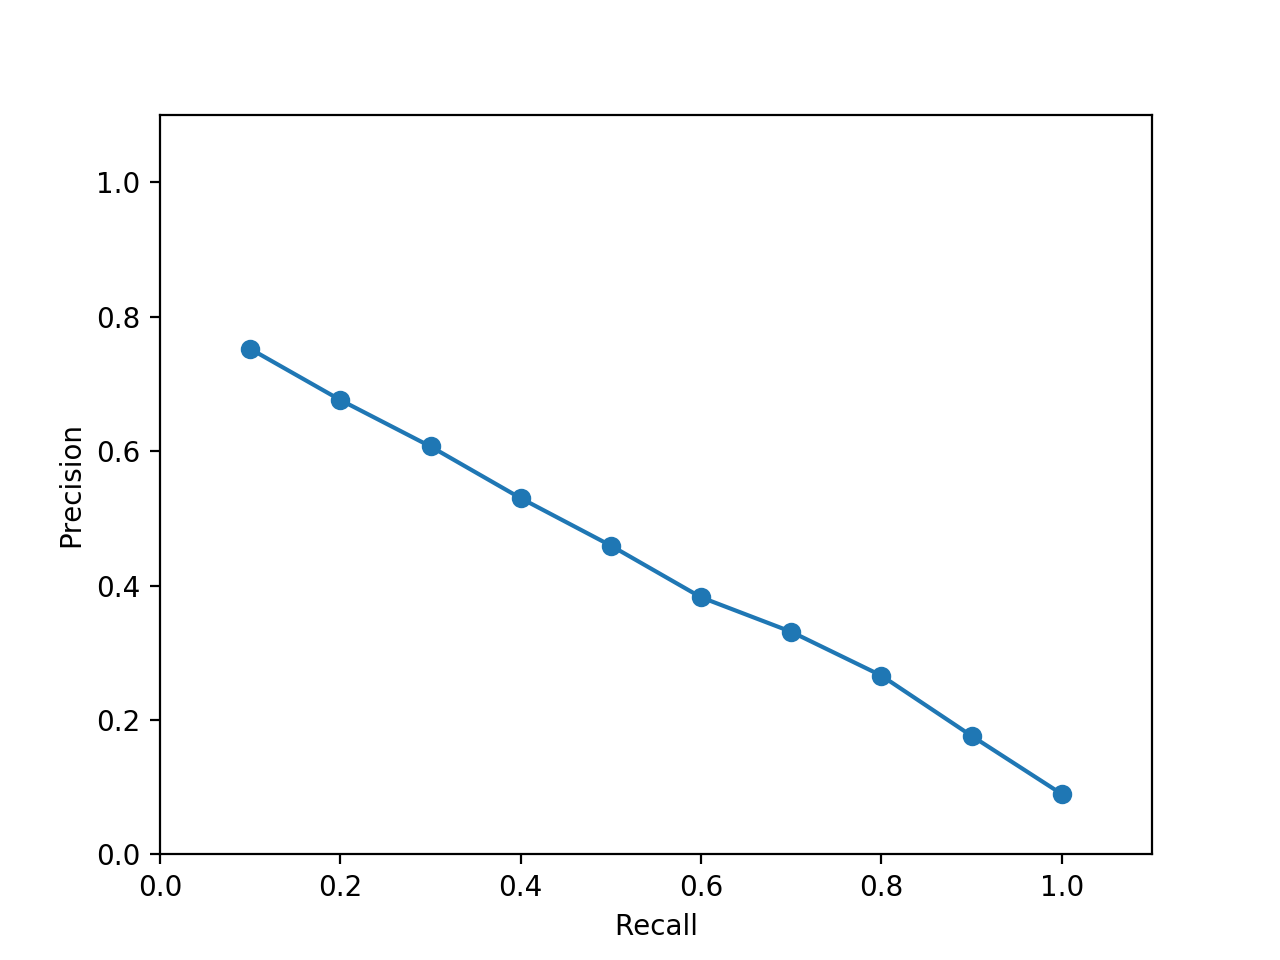
\includegraphics[totalheight=8cm]{cs.png}
%    \caption{Precision-Recall GVSM:  query , doc}
%    \label{fig:plot  }
%\end{figure}
%

\section{Future work}
In order to make the score function faster, each computation could be done in a multithreading context.\\In addition to this the term-to-term similarity scores could be precomputed and stored in a global dictionary.
\begin{thebibliography}{999}

\bibitem{c1}
  George Tsatsaronis and Vicky Panagiotopoulo,
  \emph{ A Generalized Vector Space Model for Text Retrieval Based on Semantic Relatedness}.
  \\Department of Informatics Athens University of Economics and Business, 76, Patision Str., Athens, Greece,
  2009

  
\bibitem{c2}
  Pedregosa, F. and Varoquaux, G. and Gramfort, A. and Michel, V.
         and Thirion, B. and Grisel, O. and Blondel, M. and Prettenhofer, P.
         and Weiss, R. and Dubourg, V. and Vanderplas, J. and Passos, A. and
         Cournapeau, D. and Brucher, M. and Perrot, M. and Duchesnay, E.
  \emph{\\Scikit-learn: Machine Learning in {P}ython}.
  \\Journal of Machine Learning Research, volume: 12, pages: 2825--2830, year: 2011


\end{thebibliography}





\end{document}





